\documentclass[1p]{elsarticle_modified}
%\bibliographystyle{elsarticle-num}

%\usepackage[colorlinks]{hyperref}
%\usepackage{abbrmath_seonhwa} %\Abb, \Ascr, \Acal ,\Abf, \Afrak
\usepackage{amsfonts}
\usepackage{amssymb}
\usepackage{amsmath}
\usepackage{amsthm}
\usepackage{scalefnt}
\usepackage{amsbsy}
\usepackage{kotex}
\usepackage{caption}
\usepackage{subfig}
\usepackage{color}
\usepackage{graphicx}
\usepackage{xcolor} %% white, black, red, green, blue, cyan, magenta, yellow
\usepackage{float}
\usepackage{setspace}
\usepackage{hyperref}

\usepackage{tikz}
\usetikzlibrary{arrows}

\usepackage{multirow}
\usepackage{array} % fixed length table
\usepackage{hhline}

%%%%%%%%%%%%%%%%%%%%%
\makeatletter
\renewcommand*\env@matrix[1][\arraystretch]{%
	\edef\arraystretch{#1}%
	\hskip -\arraycolsep
	\let\@ifnextchar\new@ifnextchar
	\array{*\c@MaxMatrixCols c}}
\makeatother %https://tex.stackexchange.com/questions/14071/how-can-i-increase-the-line-spacing-in-a-matrix
%%%%%%%%%%%%%%%

\usepackage[normalem]{ulem}

\newcommand{\msout}[1]{\ifmmode\text{\sout{\ensuremath{#1}}}\else\sout{#1}\fi}
%SOURCE: \msout is \stkout macro in https://tex.stackexchange.com/questions/20609/strikeout-in-math-mode

\newcommand{\cancel}[1]{
	\ifmmode
	{\color{red}\msout{#1}}
	\else
	{\color{red}\sout{#1}}
	\fi
}

\newcommand{\add}[1]{
	{\color{blue}\uwave{#1}}
}

\newcommand{\replace}[2]{
	\ifmmode
	{\color{red}\msout{#1}}{\color{blue}\uwave{#2}}
	\else
	{\color{red}\sout{#1}}{\color{blue}\uwave{#2}}
	\fi
}

\newcommand{\Sol}{\mathcal{S}} %segment
\newcommand{\D}{D} %diagram
\newcommand{\A}{\mathcal{A}} %arc


%%%%%%%%%%%%%%%%%%%%%%%%%%%%%5 test

\def\sl{\operatorname{\textup{SL}}(2,\Cbb)}
\def\psl{\operatorname{\textup{PSL}}(2,\Cbb)}
\def\quan{\mkern 1mu \triangleright \mkern 1mu}

\theoremstyle{definition}
\newtheorem{thm}{Theorem}[section]
\newtheorem{prop}[thm]{Proposition}
\newtheorem{lem}[thm]{Lemma}
\newtheorem{ques}[thm]{Question}
\newtheorem{cor}[thm]{Corollary}
\newtheorem{defn}[thm]{Definition}
\newtheorem{exam}[thm]{Example}
\newtheorem{rmk}[thm]{Remark}
\newtheorem{alg}[thm]{Algorithm}

\newcommand{\I}{\sqrt{-1}}
\begin{document}

%\begin{frontmatter}
%
%\title{Boundary parabolic representations of knots up to 8 crossings}
%
%%% Group authors per affiliation:
%\author{Yunhi Cho} 
%\address{Department of Mathematics, University of Seoul, Seoul, Korea}
%\ead{yhcho@uos.ac.kr}
%
%
%\author{Seonhwa Kim} %\fnref{s_kim}}
%\address{Center for Geometry and Physics, Institute for Basic Science, Pohang, 37673, Korea}
%\ead{ryeona17@ibs.re.kr}
%
%\author{Hyuk Kim}
%\address{Department of Mathematical Sciences, Seoul National University, Seoul 08826, Korea}
%\ead{hyukkim@snu.ac.kr}
%
%\author{Seokbeom Yoon}
%\address{Department of Mathematical Sciences, Seoul National University, Seoul, 08826,  Korea}
%\ead{sbyoon15@snu.ac.kr}
%
%\begin{abstract}
%We find all boundary parabolic representation of knots up to 8 crossings.
%
%\end{abstract}
%\begin{keyword}
%    \MSC[2010] 57M25 
%\end{keyword}
%
%\end{frontmatter}

%\linenumbers
%\tableofcontents
%
\newcommand\colored[1]{\textcolor{white}{\rule[-0.35ex]{0.8em}{1.4ex}}\kern-0.8em\color{red} #1}%
%\newcommand\colored[1]{\textcolor{white}{ #1}\kern-2.17ex	\textcolor{white}{ #1}\kern-1.81ex	\textcolor{white}{ #1}\kern-2.15ex\color{red}#1	}

{\Large $\underline{12a_{0834}~(K12a_{0834})}$}

\setlength{\tabcolsep}{10pt}
\renewcommand{\arraystretch}{1.6}
\vspace{1cm}\begin{tabular}{m{100pt}>{\centering\arraybackslash}m{274pt}}
\multirow{5}{120pt}{
	\centering
	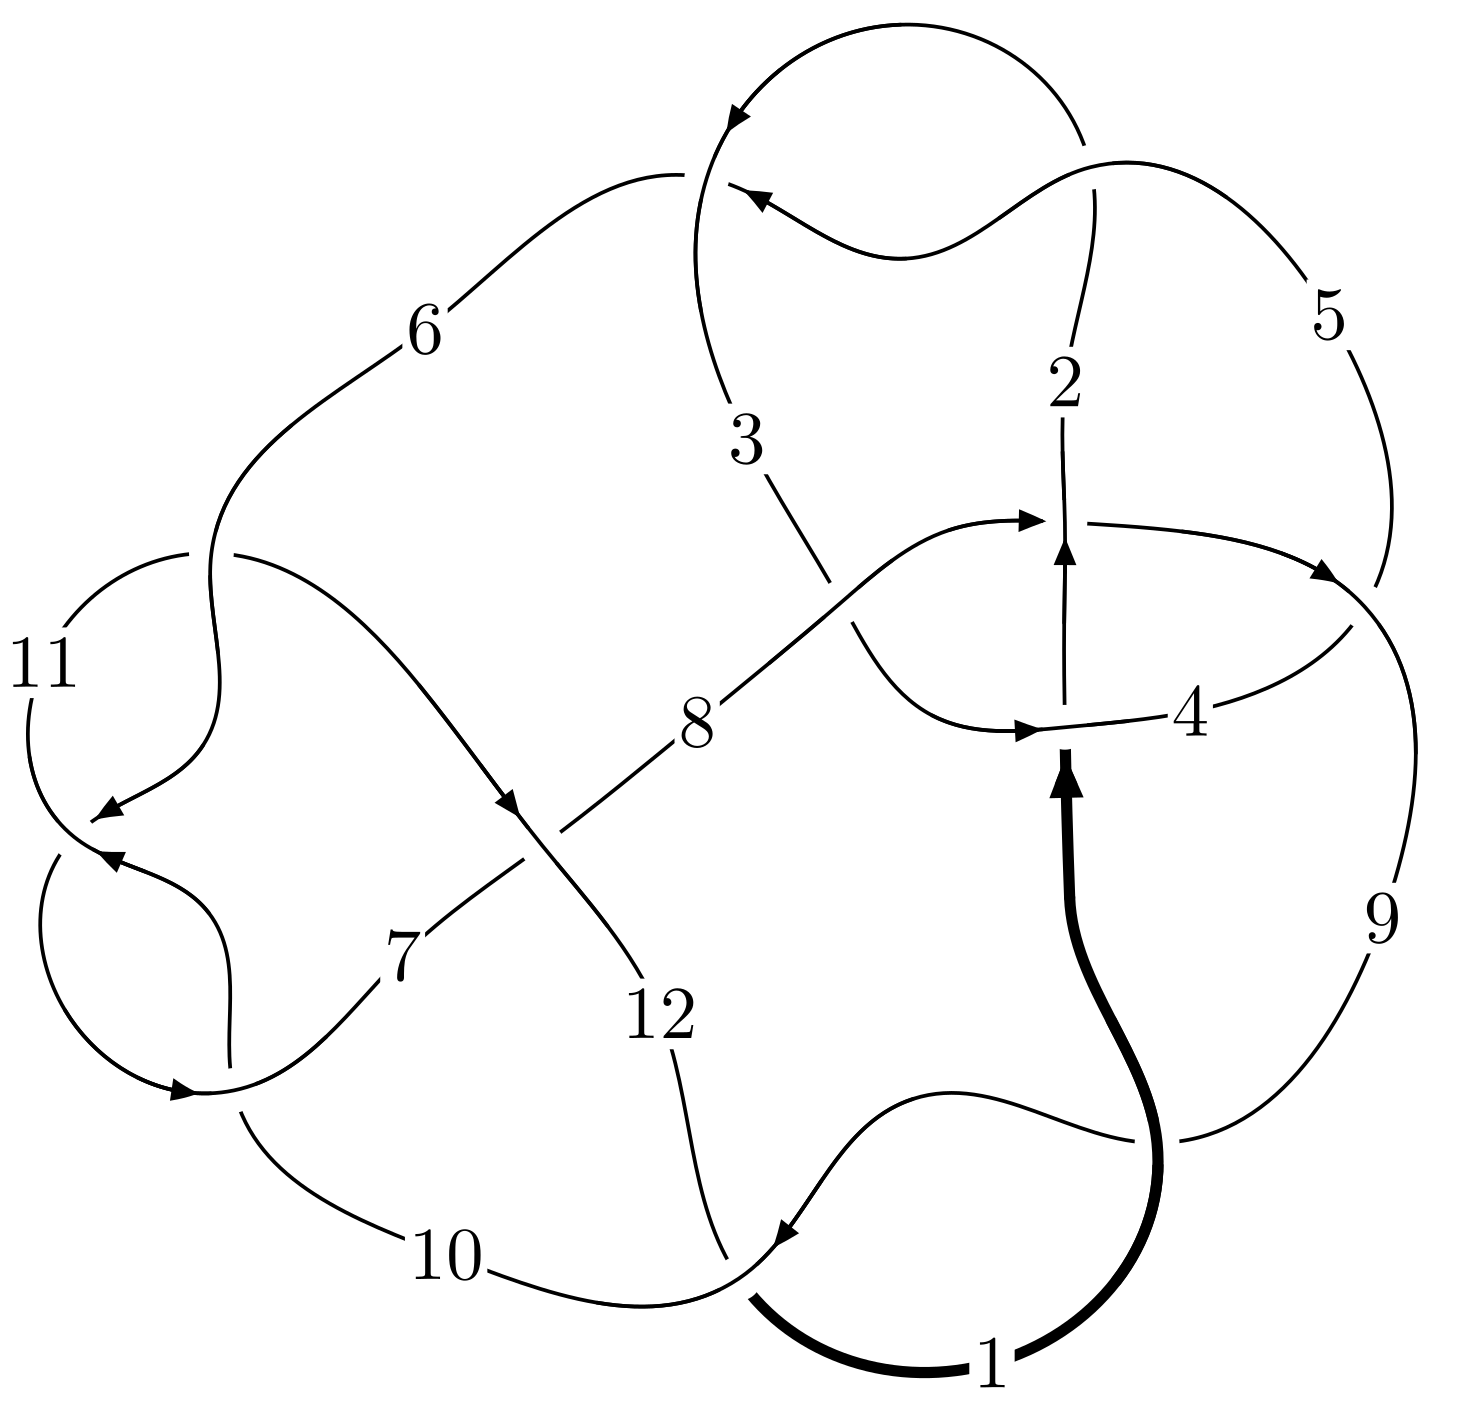
\includegraphics[width=112pt]{../../../GIT/diagram.site/Diagrams/png/1635_12a_0834.png}\\
\ \ \ A knot diagram\footnotemark}&
\allowdisplaybreaks
\textbf{Linearized knot diagam} \\
\cline{2-2}
 &
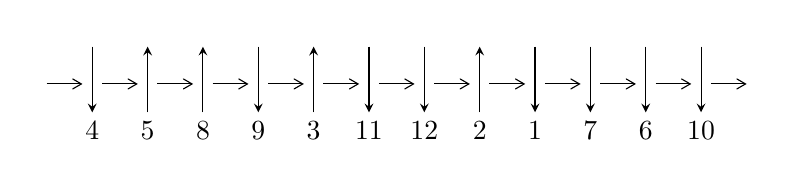
\begin{tikzpicture}[x=20pt, y=17pt]
	% nodes
	\node (C0) at (0, 0) {};
	\node (C1) at (1, 0) {};
	\node (C1U) at (1, +1) {};
	\node (C1D) at (1, -1) {4};

	\node (C2) at (2, 0) {};
	\node (C2U) at (2, +1) {};
	\node (C2D) at (2, -1) {5};

	\node (C3) at (3, 0) {};
	\node (C3U) at (3, +1) {};
	\node (C3D) at (3, -1) {8};

	\node (C4) at (4, 0) {};
	\node (C4U) at (4, +1) {};
	\node (C4D) at (4, -1) {9};

	\node (C5) at (5, 0) {};
	\node (C5U) at (5, +1) {};
	\node (C5D) at (5, -1) {3};

	\node (C6) at (6, 0) {};
	\node (C6U) at (6, +1) {};
	\node (C6D) at (6, -1) {11};

	\node (C7) at (7, 0) {};
	\node (C7U) at (7, +1) {};
	\node (C7D) at (7, -1) {12};

	\node (C8) at (8, 0) {};
	\node (C8U) at (8, +1) {};
	\node (C8D) at (8, -1) {2};

	\node (C9) at (9, 0) {};
	\node (C9U) at (9, +1) {};
	\node (C9D) at (9, -1) {1};

	\node (C10) at (10, 0) {};
	\node (C10U) at (10, +1) {};
	\node (C10D) at (10, -1) {7};

	\node (C11) at (11, 0) {};
	\node (C11U) at (11, +1) {};
	\node (C11D) at (11, -1) {6};

	\node (C12) at (12, 0) {};
	\node (C12U) at (12, +1) {};
	\node (C12D) at (12, -1) {10};
	\node (C13) at (13, 0) {};

	% arrows
	\draw[->,>={angle 60}]
	(C0) edge (C1) (C1) edge (C2) (C2) edge (C3) (C3) edge (C4) (C4) edge (C5) (C5) edge (C6) (C6) edge (C7) (C7) edge (C8) (C8) edge (C9) (C9) edge (C10) (C10) edge (C11) (C11) edge (C12) (C12) edge (C13) ;	\draw[->,>=stealth]
	(C1U) edge (C1D) (C2D) edge (C2U) (C3D) edge (C3U) (C4U) edge (C4D) (C5D) edge (C5U) (C6U) edge (C6D) (C7U) edge (C7D) (C8D) edge (C8U) (C9U) edge (C9D) (C10U) edge (C10D) (C11U) edge (C11D) (C12U) edge (C12D) ;
	\end{tikzpicture} \\
\hhline{~~} \\& 
\textbf{Solving Sequence} \\ \cline{2-2} 
 &
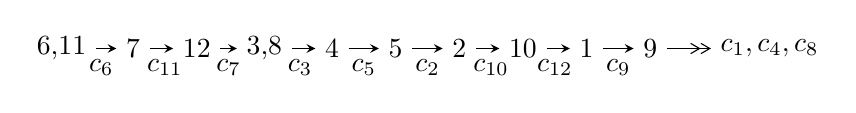
\begin{tikzpicture}[x=23pt, y=7pt]
	% node
	\node (A0) at (-1/8, 0) {6,11};
	\node (A1) at (1, 0) {7};
	\node (A2) at (2, 0) {12};
	\node (A3) at (49/16, 0) {3,8};
	\node (A4) at (33/8, 0) {4};
	\node (A5) at (41/8, 0) {5};
	\node (A6) at (49/8, 0) {2};
	\node (A7) at (57/8, 0) {10};
	\node (A8) at (65/8, 0) {1};
	\node (A9) at (73/8, 0) {9};
	\node (C1) at (1/2, -1) {$c_{6}$};
	\node (C2) at (3/2, -1) {$c_{11}$};
	\node (C3) at (5/2, -1) {$c_{7}$};
	\node (C4) at (29/8, -1) {$c_{3}$};
	\node (C5) at (37/8, -1) {$c_{5}$};
	\node (C6) at (45/8, -1) {$c_{2}$};
	\node (C7) at (53/8, -1) {$c_{10}$};
	\node (C8) at (61/8, -1) {$c_{12}$};
	\node (C9) at (69/8, -1) {$c_{9}$};
	\node (A10) at (11, 0) {$c_{1},c_{4},c_{8}$};

	% edge
	\draw[->,>=stealth]	
	(A0) edge (A1) (A1) edge (A2) (A2) edge (A3) (A3) edge (A4) (A4) edge (A5) (A5) edge (A6) (A6) edge (A7) (A7) edge (A8) (A8) edge (A9) ;
	\draw[->>,>={angle 60}]	
	(A9) edge (A10);
\end{tikzpicture} \\ 

\end{tabular} \\

\footnotetext{
The image of knot diagram is generated by the software ``\textbf{Draw programme}" developed by Andrew Bartholomew(\url{http://www.layer8.co.uk/maths/draw/index.htm\#Running-draw}), where we modified some parts for our purpose(\url{https://github.com/CATsTAILs/LinksPainter}).
}\phantom \\ \newline 
\centering \textbf{Ideals for irreducible components\footnotemark of $X_{\text{par}}$} 
 
\begin{align*}
I^u_{1}&=\langle 
-3.22741\times10^{27} u^{88}+3.46788\times10^{27} u^{87}+\cdots+1.49349\times10^{28} b+5.73350\times10^{27},\\
\phantom{I^u_{1}}&\phantom{= \langle  }8.41565\times10^{28} u^{88}-1.02242\times10^{29} u^{87}+\cdots+1.49349\times10^{28} a+2.07042\times10^{29},\;u^{89}-2 u^{88}+\cdots+u-1\rangle \\
I^u_{2}&=\langle 
b-1,\;-2 u^2+a+2 u-3,\;u^3- u^2+2 u-1\rangle \\
\\
\end{align*}
\raggedright * 2 irreducible components of $\dim_{\mathbb{C}}=0$, with total 92 representations.\\
\footnotetext{All coefficients of polynomials are rational numbers. But the coefficients are sometimes approximated in decimal forms when there is not enough margin.}
\newpage
\renewcommand{\arraystretch}{1}
\centering \section*{I. $I^u_{1}= \langle -3.23\times10^{27} u^{88}+3.47\times10^{27} u^{87}+\cdots+1.49\times10^{28} b+5.73\times10^{27},\;8.42\times10^{28} u^{88}-1.02\times10^{29} u^{87}+\cdots+1.49\times10^{28} a+2.07\times10^{29},\;u^{89}-2 u^{88}+\cdots+u-1 \rangle$}
\flushleft \textbf{(i) Arc colorings}\\
\begin{tabular}{m{7pt} m{180pt} m{7pt} m{180pt} }
\flushright $a_{6}=$&$\begin{pmatrix}1\\0\end{pmatrix}$ \\
\flushright $a_{11}=$&$\begin{pmatrix}0\\u\end{pmatrix}$ \\
\flushright $a_{7}=$&$\begin{pmatrix}1\\u^2\end{pmatrix}$ \\
\flushright $a_{12}=$&$\begin{pmatrix}- u\\u\end{pmatrix}$ \\
\flushright $a_{3}=$&$\begin{pmatrix}-5.63488 u^{88}+6.84586 u^{87}+\cdots-19.6801 u-13.8629\\0.216098 u^{88}-0.232199 u^{87}+\cdots+1.17195 u-0.383899\end{pmatrix}$ \\
\flushright $a_{8}=$&$\begin{pmatrix}- u^4- u^2+1\\u^4+2 u^2\end{pmatrix}$ \\
\flushright $a_{4}=$&$\begin{pmatrix}-4.24061 u^{88}+4.90905 u^{87}+\cdots-12.0676 u-9.67457\\1.46774 u^{88}-1.53556 u^{87}+\cdots+4.56613 u+1.46782\end{pmatrix}$ \\
\flushright $a_{5}=$&$\begin{pmatrix}5.24438 u^{88}-6.38436 u^{87}+\cdots+18.1075 u+13.9322\\-0.135606 u^{88}+0.0712031 u^{87}+\cdots-1.31220 u+0.464403\end{pmatrix}$ \\
\flushright $a_{2}=$&$\begin{pmatrix}-1.00290 u^{88}+1.84480 u^{87}+\cdots-3.68274 u-1.52239\\0.839015 u^{88}-1.67801 u^{87}+\cdots-0.719508 u+0.838993\end{pmatrix}$ \\
\flushright $a_{10}=$&$\begin{pmatrix}u\\u^3+u\end{pmatrix}$ \\
\flushright $a_{1}=$&$\begin{pmatrix}- u^5-2 u^3- u\\- u^7-3 u^5-2 u^3+u\end{pmatrix}$ \\
\flushright $a_{9}=$&$\begin{pmatrix}u^9+4 u^7+5 u^5+2 u^3+u\\u^{11}+5 u^9+8 u^7+3 u^5- u^3+u\end{pmatrix}$\\&\end{tabular}
\flushleft \textbf{(ii) Obstruction class $= -1$}\\~\\
\flushleft \textbf{(iii) Cusp Shapes $= 6.14068 u^{88}-3.32136 u^{87}+\cdots+42.7937 u+19.8607$}\\~\\
\newpage\renewcommand{\arraystretch}{1}
\flushleft \textbf{(iv) u-Polynomials at the component}\newline \\
\begin{tabular}{m{50pt}|m{274pt}}
Crossings & \hspace{64pt}u-Polynomials at each crossing \\
\hline $$\begin{aligned}c_{1}\end{aligned}$$&$\begin{aligned}
&u^{89}-15 u^{88}+\cdots+36 u-8
\end{aligned}$\\
\hline $$\begin{aligned}c_{2},c_{5}\end{aligned}$$&$\begin{aligned}
&u^{89}+4 u^{88}+\cdots+20 u+1
\end{aligned}$\\
\hline $$\begin{aligned}c_{3}\end{aligned}$$&$\begin{aligned}
&u^{89}+u^{88}+\cdots+1421584 u+441313
\end{aligned}$\\
\hline $$\begin{aligned}c_{4}\end{aligned}$$&$\begin{aligned}
&u^{89}- u^{88}+\cdots+6214 u+1559
\end{aligned}$\\
\hline $$\begin{aligned}c_{6},c_{10},c_{11}\end{aligned}$$&$\begin{aligned}
&u^{89}+2 u^{88}+\cdots+u+1
\end{aligned}$\\
\hline $$\begin{aligned}c_{7}\end{aligned}$$&$\begin{aligned}
&u^{89}-2 u^{88}+\cdots-13911 u+4113
\end{aligned}$\\
\hline $$\begin{aligned}c_{8}\end{aligned}$$&$\begin{aligned}
&u^{89}-4 u^{88}+\cdots- u+1
\end{aligned}$\\
\hline $$\begin{aligned}c_{9},c_{12}\end{aligned}$$&$\begin{aligned}
&u^{89}-12 u^{88}+\cdots-1943 u+163
\end{aligned}$\\
\hline
\end{tabular}\\~\\
\newpage\renewcommand{\arraystretch}{1}
\flushleft \textbf{(v) Riley Polynomials at the component}\newline \\
\begin{tabular}{m{50pt}|m{274pt}}
Crossings & \hspace{64pt}Riley Polynomials at each crossing \\
\hline $$\begin{aligned}c_{1}\end{aligned}$$&$\begin{aligned}
&y^{89}+21 y^{88}+\cdots-560 y-64
\end{aligned}$\\
\hline $$\begin{aligned}c_{2},c_{5}\end{aligned}$$&$\begin{aligned}
&y^{89}-70 y^{88}+\cdots+348 y-1
\end{aligned}$\\
\hline $$\begin{aligned}c_{3}\end{aligned}$$&$\begin{aligned}
&y^{89}+39 y^{88}+\cdots+7318297870790 y-194757163969
\end{aligned}$\\
\hline $$\begin{aligned}c_{4}\end{aligned}$$&$\begin{aligned}
&y^{89}+111 y^{88}+\cdots-44278234 y-2430481
\end{aligned}$\\
\hline $$\begin{aligned}c_{6},c_{10},c_{11}\end{aligned}$$&$\begin{aligned}
&y^{89}+84 y^{88}+\cdots+7 y-1
\end{aligned}$\\
\hline $$\begin{aligned}c_{7}\end{aligned}$$&$\begin{aligned}
&y^{89}+36 y^{88}+\cdots-395194221 y-16916769
\end{aligned}$\\
\hline $$\begin{aligned}c_{8}\end{aligned}$$&$\begin{aligned}
&y^{89}-16 y^{88}+\cdots+7 y-1
\end{aligned}$\\
\hline $$\begin{aligned}c_{9},c_{12}\end{aligned}$$&$\begin{aligned}
&y^{89}+84 y^{88}+\cdots+271727 y-26569
\end{aligned}$\\
\hline
\end{tabular}\\~\\
\newpage\flushleft \textbf{(vi) Complex Volumes and Cusp Shapes}
$$\begin{array}{c|c|c}  
\text{Solutions to }I^u_{1}& \I (\text{vol} + \sqrt{-1}CS) & \text{Cusp shape}\\
 \hline 
\begin{aligned}
u &= \phantom{-}0.186824 + 1.001010 I \\
a &= -0.553297 - 0.442816 I \\
b &= \phantom{-}1.183560 - 0.268162 I\end{aligned}
 & \phantom{-}3.51936 - 4.77245 I & \phantom{-0.000000 } 0 \\ \hline\begin{aligned}
u &= \phantom{-}0.186824 - 1.001010 I \\
a &= -0.553297 + 0.442816 I \\
b &= \phantom{-}1.183560 + 0.268162 I\end{aligned}
 & \phantom{-}3.51936 + 4.77245 I & \phantom{-0.000000 } 0 \\ \hline\begin{aligned}
u &= -0.620945 + 0.565816 I \\
a &= -1.037750 + 0.358176 I \\
b &= \phantom{-}1.302120 - 0.095640 I\end{aligned}
 & \phantom{-}8.53612 - 0.43548 I & \phantom{-}4.95570 + 0. I\phantom{ +0.000000I} \\ \hline\begin{aligned}
u &= -0.620945 - 0.565816 I \\
a &= -1.037750 - 0.358176 I \\
b &= \phantom{-}1.302120 + 0.095640 I\end{aligned}
 & \phantom{-}8.53612 + 0.43548 I & \phantom{-}4.95570 + 0. I\phantom{ +0.000000I} \\ \hline\begin{aligned}
u &= -0.720530 + 0.429057 I \\
a &= -0.91242 + 1.45256 I \\
b &= \phantom{-}1.288110 + 0.140305 I\end{aligned}
 & \phantom{-}8.04617 + 4.93945 I & \phantom{-}3.54197 - 5.91371 I \\ \hline\begin{aligned}
u &= -0.720530 - 0.429057 I \\
a &= -0.91242 - 1.45256 I \\
b &= \phantom{-}1.288110 - 0.140305 I\end{aligned}
 & \phantom{-}8.04617 - 4.93945 I & \phantom{-}3.54197 + 5.91371 I \\ \hline\begin{aligned}
u &= -0.199195 + 0.809899 I \\
a &= -0.636456 + 0.180505 I \\
b &= \phantom{-}1.241680 - 0.317786 I\end{aligned}
 & \phantom{-}3.66713 - 4.80341 I & \phantom{-0.000000 -}0. + 4.71638 I \\ \hline\begin{aligned}
u &= -0.199195 - 0.809899 I \\
a &= -0.636456 - 0.180505 I \\
b &= \phantom{-}1.241680 + 0.317786 I\end{aligned}
 & \phantom{-}3.66713 + 4.80341 I & \phantom{-0.000000 } 0. - 4.71638 I \\ \hline\begin{aligned}
u &= \phantom{-}0.706611 + 0.428170 I \\
a &= -1.40688 - 1.84307 I \\
b &= \phantom{-}1.45020 - 0.50983 I\end{aligned}
 & \phantom{-}8.7954 - 13.3610 I & \phantom{-0.000000 -}0. + 8.90502 I \\ \hline\begin{aligned}
u &= \phantom{-}0.706611 - 0.428170 I \\
a &= -1.40688 + 1.84307 I \\
b &= \phantom{-}1.45020 + 0.50983 I\end{aligned}
 & \phantom{-}8.7954 + 13.3610 I & \phantom{-0.000000 } 0. - 8.90502 I\\
 \hline 
 \end{array}$$\newpage$$\begin{array}{c|c|c}  
\text{Solutions to }I^u_{1}& \I (\text{vol} + \sqrt{-1}CS) & \text{Cusp shape}\\
 \hline 
\begin{aligned}
u &= \phantom{-}0.616128 + 0.547042 I \\
a &= -1.031070 - 0.355615 I \\
b &= \phantom{-}1.45184 + 0.48379 I\end{aligned}
 & \phantom{-}9.23088 + 8.93550 I & \phantom{-}1.46945 - 3.15188 I \\ \hline\begin{aligned}
u &= \phantom{-}0.616128 - 0.547042 I \\
a &= -1.031070 + 0.355615 I \\
b &= \phantom{-}1.45184 - 0.48379 I\end{aligned}
 & \phantom{-}9.23088 - 8.93550 I & \phantom{-}1.46945 + 3.15188 I \\ \hline\begin{aligned}
u &= -0.048243 + 1.175430 I \\
a &= -0.829588 + 0.561532 I \\
b &= \phantom{-}0.220153 + 0.721163 I\end{aligned}
 & \phantom{-}0.493634 - 1.143620 I & \phantom{-0.000000 } 0 \\ \hline\begin{aligned}
u &= -0.048243 - 1.175430 I \\
a &= -0.829588 - 0.561532 I \\
b &= \phantom{-}0.220153 - 0.721163 I\end{aligned}
 & \phantom{-}0.493634 + 1.143620 I & \phantom{-0.000000 } 0 \\ \hline\begin{aligned}
u &= \phantom{-}0.653621 + 0.454879 I \\
a &= \phantom{-}1.68141 + 1.55340 I \\
b &= -1.56986 + 0.64185 I\end{aligned}
 & \phantom{-}7.92409 - 4.26600 I & \phantom{-}4.93804 + 6.41768 I \\ \hline\begin{aligned}
u &= \phantom{-}0.653621 - 0.454879 I \\
a &= \phantom{-}1.68141 - 1.55340 I \\
b &= -1.56986 - 0.64185 I\end{aligned}
 & \phantom{-}7.92409 + 4.26600 I & \phantom{-}4.93804 - 6.41768 I \\ \hline\begin{aligned}
u &= \phantom{-}0.668755 + 0.428865 I \\
a &= \phantom{-}1.230110 + 0.273390 I \\
b &= -0.183511 + 1.236830 I\end{aligned}
 & \phantom{-}3.64043 - 7.32953 I & -1.17277 + 8.99350 I \\ \hline\begin{aligned}
u &= \phantom{-}0.668755 - 0.428865 I \\
a &= \phantom{-}1.230110 - 0.273390 I \\
b &= -0.183511 - 1.236830 I\end{aligned}
 & \phantom{-}3.64043 + 7.32953 I & -1.17277 - 8.99350 I \\ \hline\begin{aligned}
u &= \phantom{-}0.635432 + 0.474349 I \\
a &= \phantom{-}0.822221 + 0.986528 I \\
b &= -1.59447 - 0.59522 I\end{aligned}
 & \phantom{-}8.00335 + 0.00682 I & \phantom{-}5.30054 + 0. I\phantom{ +0.000000I} \\ \hline\begin{aligned}
u &= \phantom{-}0.635432 - 0.474349 I \\
a &= \phantom{-}0.822221 - 0.986528 I \\
b &= -1.59447 + 0.59522 I\end{aligned}
 & \phantom{-}8.00335 - 0.00682 I & \phantom{-}5.30054 + 0. I\phantom{ +0.000000I}\\
 \hline 
 \end{array}$$\newpage$$\begin{array}{c|c|c}  
\text{Solutions to }I^u_{1}& \I (\text{vol} + \sqrt{-1}CS) & \text{Cusp shape}\\
 \hline 
\begin{aligned}
u &= \phantom{-}0.605334 + 0.494722 I \\
a &= -0.648146 + 0.252052 I \\
b &= -0.237306 - 1.205620 I\end{aligned}
 & \phantom{-}3.91183 + 3.11100 I & -0.25921 - 2.86336 I \\ \hline\begin{aligned}
u &= \phantom{-}0.605334 - 0.494722 I \\
a &= -0.648146 - 0.252052 I \\
b &= -0.237306 + 1.205620 I\end{aligned}
 & \phantom{-}3.91183 - 3.11100 I & -0.25921 + 2.86336 I \\ \hline\begin{aligned}
u &= -0.631916 + 0.451263 I \\
a &= \phantom{-}3.21792 - 1.12316 I \\
b &= -1.134390 - 0.014055 I\end{aligned}
 & \phantom{-}5.44595 + 2.07449 I & -17.7402 - 1.7776 I \\ \hline\begin{aligned}
u &= -0.631916 - 0.451263 I \\
a &= \phantom{-}3.21792 + 1.12316 I \\
b &= -1.134390 + 0.014055 I\end{aligned}
 & \phantom{-}5.44595 - 2.07449 I & -17.7402 + 1.7776 I \\ \hline\begin{aligned}
u &= -0.646012 + 0.423346 I \\
a &= -0.072596 - 0.739156 I \\
b &= -0.223514 - 0.368374 I\end{aligned}
 & \phantom{-}3.49478 + 3.09238 I & -1.72304 - 2.11901 I \\ \hline\begin{aligned}
u &= -0.646012 - 0.423346 I \\
a &= -0.072596 + 0.739156 I \\
b &= -0.223514 + 0.368374 I\end{aligned}
 & \phantom{-}3.49478 - 3.09238 I & -1.72304 + 2.11901 I \\ \hline\begin{aligned}
u &= -0.599733 + 0.464946 I \\
a &= -0.636254 + 0.368078 I \\
b &= -0.299671 + 0.334219 I\end{aligned}
 & \phantom{-}3.68292 + 0.99040 I & -0.83517 - 4.70946 I \\ \hline\begin{aligned}
u &= -0.599733 - 0.464946 I \\
a &= -0.636254 - 0.368078 I \\
b &= -0.299671 - 0.334219 I\end{aligned}
 & \phantom{-}3.68292 - 0.99040 I & -0.83517 + 4.70946 I \\ \hline\begin{aligned}
u &= \phantom{-}0.718124 + 0.121384 I \\
a &= \phantom{-}0.696924 - 0.479554 I \\
b &= \phantom{-}1.147890 + 0.156346 I\end{aligned}
 & \phantom{-}0.82958 + 1.21576 I & \phantom{-}0.08046 - 5.50881 I \\ \hline\begin{aligned}
u &= \phantom{-}0.718124 - 0.121384 I \\
a &= \phantom{-}0.696924 + 0.479554 I \\
b &= \phantom{-}1.147890 - 0.156346 I\end{aligned}
 & \phantom{-}0.82958 - 1.21576 I & \phantom{-}0.08046 + 5.50881 I\\
 \hline 
 \end{array}$$\newpage$$\begin{array}{c|c|c}  
\text{Solutions to }I^u_{1}& \I (\text{vol} + \sqrt{-1}CS) & \text{Cusp shape}\\
 \hline 
\begin{aligned}
u &= -0.684438 + 0.175505 I \\
a &= \phantom{-}0.26626 + 1.65738 I \\
b &= \phantom{-}1.267190 + 0.412877 I\end{aligned}
 & \phantom{-}1.50927 + 8.27164 I & -3.69410 - 8.67253 I \\ \hline\begin{aligned}
u &= -0.684438 - 0.175505 I \\
a &= \phantom{-}0.26626 - 1.65738 I \\
b &= \phantom{-}1.267190 - 0.412877 I\end{aligned}
 & \phantom{-}1.50927 - 8.27164 I & -3.69410 + 8.67253 I \\ \hline\begin{aligned}
u &= \phantom{-}0.153919 + 1.287670 I \\
a &= -0.556228 + 0.142914 I \\
b &= \phantom{-}0.047805 + 0.139825 I\end{aligned}
 & \phantom{-}2.98737 - 2.41032 I & \phantom{-0.000000 } 0 \\ \hline\begin{aligned}
u &= \phantom{-}0.153919 - 1.287670 I \\
a &= -0.556228 - 0.142914 I \\
b &= \phantom{-}0.047805 - 0.139825 I\end{aligned}
 & \phantom{-}2.98737 + 2.41032 I & \phantom{-0.000000 } 0 \\ \hline\begin{aligned}
u &= \phantom{-}0.080784 + 1.301410 I \\
a &= -0.81013 - 1.51262 I \\
b &= -0.751023 - 0.026185 I\end{aligned}
 & \phantom{-}4.46740 - 1.57474 I & \phantom{-0.000000 } 0 \\ \hline\begin{aligned}
u &= \phantom{-}0.080784 - 1.301410 I \\
a &= -0.81013 + 1.51262 I \\
b &= -0.751023 + 0.026185 I\end{aligned}
 & \phantom{-}4.46740 + 1.57474 I & \phantom{-0.000000 } 0 \\ \hline\begin{aligned}
u &= \phantom{-}0.132994 + 1.322700 I \\
a &= \phantom{-}3.11220 + 4.00074 I \\
b &= -1.009110 + 0.076392 I\end{aligned}
 & \phantom{-}5.08256 - 2.31872 I & \phantom{-0.000000 } 0 \\ \hline\begin{aligned}
u &= \phantom{-}0.132994 - 1.322700 I \\
a &= \phantom{-}3.11220 - 4.00074 I \\
b &= -1.009110 - 0.076392 I\end{aligned}
 & \phantom{-}5.08256 + 2.31872 I & \phantom{-0.000000 } 0 \\ \hline\begin{aligned}
u &= -0.199595 + 1.316790 I \\
a &= \phantom{-}0.750885 - 0.065218 I \\
b &= \phantom{-}0.029505 - 1.017910 I\end{aligned}
 & \phantom{-}2.22525 + 6.49294 I & \phantom{-0.000000 } 0 \\ \hline\begin{aligned}
u &= -0.199595 - 1.316790 I \\
a &= \phantom{-}0.750885 + 0.065218 I \\
b &= \phantom{-}0.029505 + 1.017910 I\end{aligned}
 & \phantom{-}2.22525 - 6.49294 I & \phantom{-0.000000 } 0\\
 \hline 
 \end{array}$$\newpage$$\begin{array}{c|c|c}  
\text{Solutions to }I^u_{1}& \I (\text{vol} + \sqrt{-1}CS) & \text{Cusp shape}\\
 \hline 
\begin{aligned}
u &= \phantom{-}0.291643 + 1.302160 I \\
a &= -0.743264 - 1.113150 I \\
b &= \phantom{-}1.143230 + 0.075944 I\end{aligned}
 & \phantom{-}5.26574 - 2.44320 I & \phantom{-0.000000 } 0 \\ \hline\begin{aligned}
u &= \phantom{-}0.291643 - 1.302160 I \\
a &= -0.743264 + 1.113150 I \\
b &= \phantom{-}1.143230 - 0.075944 I\end{aligned}
 & \phantom{-}5.26574 + 2.44320 I & \phantom{-0.000000 } 0 \\ \hline\begin{aligned}
u &= -0.035448 + 1.346970 I \\
a &= -0.289975 - 0.454139 I \\
b &= -0.555222 + 0.719411 I\end{aligned}
 & \phantom{-}4.96955 - 1.39741 I & \phantom{-0.000000 } 0 \\ \hline\begin{aligned}
u &= -0.035448 - 1.346970 I \\
a &= -0.289975 + 0.454139 I \\
b &= -0.555222 - 0.719411 I\end{aligned}
 & \phantom{-}4.96955 + 1.39741 I & \phantom{-0.000000 } 0 \\ \hline\begin{aligned}
u &= -0.256781 + 1.333000 I \\
a &= -1.48167 + 1.52113 I \\
b &= \phantom{-}1.302130 + 0.460891 I\end{aligned}
 & \phantom{-}6.23989 + 11.67750 I & \phantom{-0.000000 } 0 \\ \hline\begin{aligned}
u &= -0.256781 - 1.333000 I \\
a &= -1.48167 - 1.52113 I \\
b &= \phantom{-}1.302130 - 0.460891 I\end{aligned}
 & \phantom{-}6.23989 - 11.67750 I & \phantom{-0.000000 } 0 \\ \hline\begin{aligned}
u &= -0.158173 + 1.352240 I \\
a &= \phantom{-}1.53661 - 1.34959 I \\
b &= -1.220590 - 0.636233 I\end{aligned}
 & \phantom{-}6.70286 + 4.62002 I & \phantom{-0.000000 } 0 \\ \hline\begin{aligned}
u &= -0.158173 - 1.352240 I \\
a &= \phantom{-}1.53661 + 1.34959 I \\
b &= -1.220590 + 0.636233 I\end{aligned}
 & \phantom{-}6.70286 - 4.62002 I & \phantom{-0.000000 } 0 \\ \hline\begin{aligned}
u &= -0.107849 + 1.363370 I \\
a &= \phantom{-}1.75828 - 0.87708 I \\
b &= -1.48488 + 0.23340 I\end{aligned}
 & \phantom{-}7.55333 + 1.23341 I & \phantom{-0.000000 } 0 \\ \hline\begin{aligned}
u &= -0.107849 - 1.363370 I \\
a &= \phantom{-}1.75828 + 0.87708 I \\
b &= -1.48488 - 0.23340 I\end{aligned}
 & \phantom{-}7.55333 - 1.23341 I & \phantom{-0.000000 } 0\\
 \hline 
 \end{array}$$\newpage$$\begin{array}{c|c|c}  
\text{Solutions to }I^u_{1}& \I (\text{vol} + \sqrt{-1}CS) & \text{Cusp shape}\\
 \hline 
\begin{aligned}
u &= \phantom{-}0.567953 + 0.227198 I \\
a &= -1.15850 - 0.86882 I \\
b &= \phantom{-}0.347206 - 0.379172 I\end{aligned}
 & -1.52582 - 0.95700 I & -9.87795 + 4.21075 I \\ \hline\begin{aligned}
u &= \phantom{-}0.567953 - 0.227198 I \\
a &= -1.15850 + 0.86882 I \\
b &= \phantom{-}0.347206 + 0.379172 I\end{aligned}
 & -1.52582 + 0.95700 I & -9.87795 - 4.21075 I \\ \hline\begin{aligned}
u &= -0.591935 + 0.127305 I \\
a &= \phantom{-}0.34472 - 1.48165 I \\
b &= \phantom{-}0.060856 - 0.888636 I\end{aligned}
 & -2.27566 + 3.62056 I & -9.44307 - 7.65821 I \\ \hline\begin{aligned}
u &= -0.591935 - 0.127305 I \\
a &= \phantom{-}0.34472 + 1.48165 I \\
b &= \phantom{-}0.060856 + 0.888636 I\end{aligned}
 & -2.27566 - 3.62056 I & -9.44307 + 7.65821 I \\ \hline\begin{aligned}
u &= \phantom{-}0.210272 + 1.386360 I \\
a &= -1.53349 - 0.48155 I \\
b &= \phantom{-}0.545025 - 0.309905 I\end{aligned}
 & \phantom{-}3.62716 - 3.79171 I & \phantom{-0.000000 } 0 \\ \hline\begin{aligned}
u &= \phantom{-}0.210272 - 1.386360 I \\
a &= -1.53349 + 0.48155 I \\
b &= \phantom{-}0.545025 + 0.309905 I\end{aligned}
 & \phantom{-}3.62716 + 3.79171 I & \phantom{-0.000000 } 0 \\ \hline\begin{aligned}
u &= -0.01165 + 1.46576 I \\
a &= -2.28540 + 0.25970 I \\
b &= \phantom{-}1.361610 - 0.247191 I\end{aligned}
 & \phantom{-}10.61070 - 4.48770 I & \phantom{-0.000000 } 0 \\ \hline\begin{aligned}
u &= -0.01165 - 1.46576 I \\
a &= -2.28540 - 0.25970 I \\
b &= \phantom{-}1.361610 + 0.247191 I\end{aligned}
 & \phantom{-}10.61070 + 4.48770 I & \phantom{-0.000000 } 0 \\ \hline\begin{aligned}
u &= \phantom{-}0.516833\phantom{ +0.000000I} \\
a &= -0.695251\phantom{ +0.000000I} \\
b &= \phantom{-}0.0489090\phantom{ +0.000000I}\end{aligned}
 & -1.00847\phantom{ +0.000000I} & -9.89690\phantom{ +0.000000I} \\ \hline\begin{aligned}
u &= -0.23769 + 1.46614 I \\
a &= \phantom{-}0.195432 - 0.315957 I \\
b &= -0.213629 - 0.424957 I\end{aligned}
 & \phantom{-}9.58671 + 6.32782 I & \phantom{-0.000000 } 0\\
 \hline 
 \end{array}$$\newpage$$\begin{array}{c|c|c}  
\text{Solutions to }I^u_{1}& \I (\text{vol} + \sqrt{-1}CS) & \text{Cusp shape}\\
 \hline 
\begin{aligned}
u &= -0.23769 - 1.46614 I \\
a &= \phantom{-}0.195432 + 0.315957 I \\
b &= -0.213629 + 0.424957 I\end{aligned}
 & \phantom{-}9.58671 - 6.32782 I & \phantom{-0.000000 } 0 \\ \hline\begin{aligned}
u &= -0.21562 + 1.47090 I \\
a &= -0.262181 + 0.065389 I \\
b &= -0.352537 + 0.382462 I\end{aligned}
 & \phantom{-}9.91923 + 3.97356 I & \phantom{-0.000000 } 0 \\ \hline\begin{aligned}
u &= -0.21562 - 1.47090 I \\
a &= -0.262181 - 0.065389 I \\
b &= -0.352537 - 0.382462 I\end{aligned}
 & \phantom{-}9.91923 - 3.97356 I & \phantom{-0.000000 } 0 \\ \hline\begin{aligned}
u &= -0.476517 + 0.190593 I \\
a &= -0.67906 - 2.37641 I \\
b &= -1.100380 - 0.487121 I\end{aligned}
 & \phantom{-}1.85802 + 2.29172 I & -0.53042 - 8.83653 I \\ \hline\begin{aligned}
u &= -0.476517 - 0.190593 I \\
a &= -0.67906 + 2.37641 I \\
b &= -1.100380 + 0.487121 I\end{aligned}
 & \phantom{-}1.85802 - 2.29172 I & -0.53042 + 8.83653 I \\ \hline\begin{aligned}
u &= -0.22812 + 1.47310 I \\
a &= \phantom{-}3.94764 - 1.14819 I \\
b &= -1.153190 - 0.026940 I\end{aligned}
 & \phantom{-}11.65640 + 5.21992 I & \phantom{-0.000000 } 0 \\ \hline\begin{aligned}
u &= -0.22812 - 1.47310 I \\
a &= \phantom{-}3.94764 + 1.14819 I \\
b &= -1.153190 + 0.026940 I\end{aligned}
 & \phantom{-}11.65640 - 5.21992 I & \phantom{-0.000000 } 0 \\ \hline\begin{aligned}
u &= \phantom{-}0.24459 + 1.47168 I \\
a &= \phantom{-}1.35920 - 0.87240 I \\
b &= -0.174652 + 1.279720 I\end{aligned}
 & \phantom{-}9.7752 - 10.6673 I & \phantom{-0.000000 } 0 \\ \hline\begin{aligned}
u &= \phantom{-}0.24459 - 1.47168 I \\
a &= \phantom{-}1.35920 + 0.87240 I \\
b &= -0.174652 - 1.279720 I\end{aligned}
 & \phantom{-}9.7752 + 10.6673 I & \phantom{-0.000000 } 0 \\ \hline\begin{aligned}
u &= \phantom{-}0.21041 + 1.48030 I \\
a &= -0.356488 + 1.319030 I \\
b &= -0.289225 - 1.238400 I\end{aligned}
 & \phantom{-}10.28920 + 0.14526 I & \phantom{-0.000000 } 0\\
 \hline 
 \end{array}$$\newpage$$\begin{array}{c|c|c}  
\text{Solutions to }I^u_{1}& \I (\text{vol} + \sqrt{-1}CS) & \text{Cusp shape}\\
 \hline 
\begin{aligned}
u &= \phantom{-}0.21041 - 1.48030 I \\
a &= -0.356488 - 1.319030 I \\
b &= -0.289225 + 1.238400 I\end{aligned}
 & \phantom{-}10.28920 - 0.14526 I & \phantom{-0.000000 } 0 \\ \hline\begin{aligned}
u &= \phantom{-}0.23458 + 1.47832 I \\
a &= \phantom{-}3.00495 + 0.89538 I \\
b &= -1.58752 + 0.68020 I\end{aligned}
 & \phantom{-}14.1722 - 7.5096 I & \phantom{-0.000000 } 0 \\ \hline\begin{aligned}
u &= \phantom{-}0.23458 - 1.47832 I \\
a &= \phantom{-}3.00495 - 0.89538 I \\
b &= -1.58752 - 0.68020 I\end{aligned}
 & \phantom{-}14.1722 + 7.5096 I & \phantom{-0.000000 } 0 \\ \hline\begin{aligned}
u &= \phantom{-}0.22444 + 1.48115 I \\
a &= \phantom{-}2.23509 + 1.47442 I \\
b &= -1.64007 - 0.59040 I\end{aligned}
 & \phantom{-}14.3257 - 3.1289 I & \phantom{-0.000000 } 0 \\ \hline\begin{aligned}
u &= \phantom{-}0.22444 - 1.48115 I \\
a &= \phantom{-}2.23509 - 1.47442 I \\
b &= -1.64007 + 0.59040 I\end{aligned}
 & \phantom{-}14.3257 + 3.1289 I & \phantom{-0.000000 } 0 \\ \hline\begin{aligned}
u &= \phantom{-}0.25953 + 1.47721 I \\
a &= -2.68774 - 1.36381 I \\
b &= \phantom{-}1.46198 - 0.52526 I\end{aligned}
 & \phantom{-}14.9486 - 16.8872 I & \phantom{-0.000000 } 0 \\ \hline\begin{aligned}
u &= \phantom{-}0.25953 - 1.47721 I \\
a &= -2.68774 + 1.36381 I \\
b &= \phantom{-}1.46198 + 0.52526 I\end{aligned}
 & \phantom{-}14.9486 + 16.8872 I & \phantom{-0.000000 } 0 \\ \hline\begin{aligned}
u &= -0.26452 + 1.48015 I \\
a &= -2.09557 + 1.31067 I \\
b &= \phantom{-}1.303210 + 0.172877 I\end{aligned}
 & \phantom{-}14.2145 + 8.5330 I & \phantom{-0.000000 } 0 \\ \hline\begin{aligned}
u &= -0.26452 - 1.48015 I \\
a &= -2.09557 - 1.31067 I \\
b &= \phantom{-}1.303210 - 0.172877 I\end{aligned}
 & \phantom{-}14.2145 - 8.5330 I & \phantom{-0.000000 } 0 \\ \hline\begin{aligned}
u &= \phantom{-}0.19817 + 1.49988 I \\
a &= -2.32503 - 0.71404 I \\
b &= \phantom{-}1.47701 + 0.46900 I\end{aligned}
 & \phantom{-}15.8886 + 6.0076 I & \phantom{-0.000000 } 0\\
 \hline 
 \end{array}$$\newpage$$\begin{array}{c|c|c}  
\text{Solutions to }I^u_{1}& \I (\text{vol} + \sqrt{-1}CS) & \text{Cusp shape}\\
 \hline 
\begin{aligned}
u &= \phantom{-}0.19817 - 1.49988 I \\
a &= -2.32503 + 0.71404 I \\
b &= \phantom{-}1.47701 - 0.46900 I\end{aligned}
 & \phantom{-}15.8886 - 6.0076 I & \phantom{-0.000000 } 0 \\ \hline\begin{aligned}
u &= -0.19383 + 1.50620 I \\
a &= -2.22103 + 0.36980 I \\
b &= \phantom{-}1.351270 - 0.081184 I\end{aligned}
 & \phantom{-}15.2931 + 2.4799 I & \phantom{-0.000000 } 0 \\ \hline\begin{aligned}
u &= -0.19383 - 1.50620 I \\
a &= -2.22103 - 0.36980 I \\
b &= \phantom{-}1.351270 + 0.081184 I\end{aligned}
 & \phantom{-}15.2931 - 2.4799 I & \phantom{-0.000000 } 0 \\ \hline\begin{aligned}
u &= \phantom{-}0.459004 + 0.059596 I \\
a &= -1.66860 + 5.99811 I \\
b &= -0.951109 + 0.022024 I\end{aligned}
 & \phantom{-}0.753766 - 0.203656 I & \phantom{-}22.5346 - 14.4002 I \\ \hline\begin{aligned}
u &= \phantom{-}0.459004 - 0.059596 I \\
a &= -1.66860 - 5.99811 I \\
b &= -0.951109 - 0.022024 I\end{aligned}
 & \phantom{-}0.753766 + 0.203656 I & \phantom{-}22.5346 + 14.4002 I \\ \hline\begin{aligned}
u &= \phantom{-}0.056793 + 0.423831 I \\
a &= -0.930309 - 0.128835 I \\
b &= -0.051016 + 0.551004 I\end{aligned}
 & -0.13700 - 1.45966 I & -2.24355 + 4.15647 I \\ \hline\begin{aligned}
u &= \phantom{-}0.056793 - 0.423831 I \\
a &= -0.930309 + 0.128835 I \\
b &= -0.051016 - 0.551004 I\end{aligned}
 & -0.13700 + 1.45966 I & -2.24355 - 4.15647 I \\ \hline\begin{aligned}
u &= -0.245590 + 0.252375 I \\
a &= -0.463084 - 0.961078 I \\
b &= -1.231150 + 0.180055 I\end{aligned}
 & \phantom{-}2.58237 - 0.25412 I & \phantom{-}3.14425 - 3.55228 I \\ \hline\begin{aligned}
u &= -0.245590 - 0.252375 I \\
a &= -0.463084 + 0.961078 I \\
b &= -1.231150 - 0.180055 I\end{aligned}
 & \phantom{-}2.58237 + 0.25412 I & \phantom{-}3.14425 + 3.55228 I\\
 \hline 
 \end{array}$$\newpage\newpage\renewcommand{\arraystretch}{1}
\centering \section*{II. $I^u_{2}= \langle b-1,\;-2 u^2+a+2 u-3,\;u^3- u^2+2 u-1 \rangle$}
\flushleft \textbf{(i) Arc colorings}\\
\begin{tabular}{m{7pt} m{180pt} m{7pt} m{180pt} }
\flushright $a_{6}=$&$\begin{pmatrix}1\\0\end{pmatrix}$ \\
\flushright $a_{11}=$&$\begin{pmatrix}0\\u\end{pmatrix}$ \\
\flushright $a_{7}=$&$\begin{pmatrix}1\\u^2\end{pmatrix}$ \\
\flushright $a_{12}=$&$\begin{pmatrix}- u\\u\end{pmatrix}$ \\
\flushright $a_{3}=$&$\begin{pmatrix}2 u^2-2 u+3\\1\end{pmatrix}$ \\
\flushright $a_{8}=$&$\begin{pmatrix}u\\u^2- u+1\end{pmatrix}$ \\
\flushright $a_{4}=$&$\begin{pmatrix}u^2- u+2\\0\end{pmatrix}$ \\
\flushright $a_{5}=$&$\begin{pmatrix}2 u^2-2 u+4\\1\end{pmatrix}$ \\
\flushright $a_{2}=$&$\begin{pmatrix}-1\\0\end{pmatrix}$ \\
\flushright $a_{10}=$&$\begin{pmatrix}u\\u^2- u+1\end{pmatrix}$ \\
\flushright $a_{1}=$&$\begin{pmatrix}-1\\0\end{pmatrix}$ \\
\flushright $a_{9}=$&$\begin{pmatrix}u^2+1\\u^2- u+1\end{pmatrix}$\\&\end{tabular}
\flushleft \textbf{(ii) Obstruction class $= 1$}\\~\\
\flushleft \textbf{(iii) Cusp Shapes $= - u^2+3 u-3$}\\~\\
\newpage\renewcommand{\arraystretch}{1}
\flushleft \textbf{(iv) u-Polynomials at the component}\newline \\
\begin{tabular}{m{50pt}|m{274pt}}
Crossings & \hspace{64pt}u-Polynomials at each crossing \\
\hline $$\begin{aligned}c_{1}\end{aligned}$$&$\begin{aligned}
&u^3
\end{aligned}$\\
\hline $$\begin{aligned}c_{2}\end{aligned}$$&$\begin{aligned}
&(u+1)^3
\end{aligned}$\\
\hline $$\begin{aligned}c_{3},c_{4}\end{aligned}$$&$\begin{aligned}
&u^3- u-1
\end{aligned}$\\
\hline $$\begin{aligned}c_{5}\end{aligned}$$&$\begin{aligned}
&(u-1)^3
\end{aligned}$\\
\hline $$\begin{aligned}c_{6}\end{aligned}$$&$\begin{aligned}
&u^3- u^2+2 u-1
\end{aligned}$\\
\hline $$\begin{aligned}c_{7},c_{8},c_{9}\end{aligned}$$&$\begin{aligned}
&u^3+u^2-1
\end{aligned}$\\
\hline $$\begin{aligned}c_{10},c_{11}\end{aligned}$$&$\begin{aligned}
&u^3+u^2+2 u+1
\end{aligned}$\\
\hline $$\begin{aligned}c_{12}\end{aligned}$$&$\begin{aligned}
&u^3- u^2+1
\end{aligned}$\\
\hline
\end{tabular}\\~\\
\newpage\renewcommand{\arraystretch}{1}
\flushleft \textbf{(v) Riley Polynomials at the component}\newline \\
\begin{tabular}{m{50pt}|m{274pt}}
Crossings & \hspace{64pt}Riley Polynomials at each crossing \\
\hline $$\begin{aligned}c_{1}\end{aligned}$$&$\begin{aligned}
&y^3
\end{aligned}$\\
\hline $$\begin{aligned}c_{2},c_{5}\end{aligned}$$&$\begin{aligned}
&(y-1)^3
\end{aligned}$\\
\hline $$\begin{aligned}c_{3},c_{4}\end{aligned}$$&$\begin{aligned}
&y^3-2 y^2+y-1
\end{aligned}$\\
\hline $$\begin{aligned}c_{6},c_{10},c_{11}\end{aligned}$$&$\begin{aligned}
&y^3+3 y^2+2 y-1
\end{aligned}$\\
\hline $$\begin{aligned}c_{7},c_{8},c_{9}\\c_{12}\end{aligned}$$&$\begin{aligned}
&y^3- y^2+2 y-1
\end{aligned}$\\
\hline
\end{tabular}\\~\\
\newpage\flushleft \textbf{(vi) Complex Volumes and Cusp Shapes}
$$\begin{array}{c|c|c}  
\text{Solutions to }I^u_{2}& \I (\text{vol} + \sqrt{-1}CS) & \text{Cusp shape}\\
 \hline 
\begin{aligned}
u &= \phantom{-}0.215080 + 1.307140 I \\
a &= -0.75488 - 1.48972 I \\
b &= \phantom{-}1.00000\phantom{ +0.000000I}\end{aligned}
 & \phantom{-}4.66906 - 2.82812 I & -0.69240 + 3.35914 I \\ \hline\begin{aligned}
u &= \phantom{-}0.215080 - 1.307140 I \\
a &= -0.75488 + 1.48972 I \\
b &= \phantom{-}1.00000\phantom{ +0.000000I}\end{aligned}
 & \phantom{-}4.66906 + 2.82812 I & -0.69240 - 3.35914 I \\ \hline\begin{aligned}
u &= \phantom{-}0.569840\phantom{ +0.000000I} \\
a &= \phantom{-}2.50976\phantom{ +0.000000I} \\
b &= \phantom{-}1.00000\phantom{ +0.000000I}\end{aligned}
 & \phantom{-}0.531480\phantom{ +0.000000I} & -1.61520\phantom{ +0.000000I}\\
 \hline 
 \end{array}$$\newpage
\newpage\renewcommand{\arraystretch}{1}
\centering \section*{ III. u-Polynomials}
\begin{tabular}{m{50pt}|m{274pt}}
Crossings & \hspace{64pt}u-Polynomials at each crossing \\
\hline $$\begin{aligned}c_{1}\end{aligned}$$&$\begin{aligned}
&u^3(u^{89}-15 u^{88}+\cdots+36 u-8)
\end{aligned}$\\
\hline $$\begin{aligned}c_{2}\end{aligned}$$&$\begin{aligned}
&((u+1)^3)(u^{89}+4 u^{88}+\cdots+20 u+1)
\end{aligned}$\\
\hline $$\begin{aligned}c_{3}\end{aligned}$$&$\begin{aligned}
&(u^3- u-1)(u^{89}+u^{88}+\cdots+1421584 u+441313)
\end{aligned}$\\
\hline $$\begin{aligned}c_{4}\end{aligned}$$&$\begin{aligned}
&(u^3- u-1)(u^{89}- u^{88}+\cdots+6214 u+1559)
\end{aligned}$\\
\hline $$\begin{aligned}c_{5}\end{aligned}$$&$\begin{aligned}
&((u-1)^3)(u^{89}+4 u^{88}+\cdots+20 u+1)
\end{aligned}$\\
\hline $$\begin{aligned}c_{6}\end{aligned}$$&$\begin{aligned}
&(u^3- u^2+2 u-1)(u^{89}+2 u^{88}+\cdots+u+1)
\end{aligned}$\\
\hline $$\begin{aligned}c_{7}\end{aligned}$$&$\begin{aligned}
&(u^3+u^2-1)(u^{89}-2 u^{88}+\cdots-13911 u+4113)
\end{aligned}$\\
\hline $$\begin{aligned}c_{8}\end{aligned}$$&$\begin{aligned}
&(u^3+u^2-1)(u^{89}-4 u^{88}+\cdots- u+1)
\end{aligned}$\\
\hline $$\begin{aligned}c_{9}\end{aligned}$$&$\begin{aligned}
&(u^3+u^2-1)(u^{89}-12 u^{88}+\cdots-1943 u+163)
\end{aligned}$\\
\hline $$\begin{aligned}c_{10},c_{11}\end{aligned}$$&$\begin{aligned}
&(u^3+u^2+2 u+1)(u^{89}+2 u^{88}+\cdots+u+1)
\end{aligned}$\\
\hline $$\begin{aligned}c_{12}\end{aligned}$$&$\begin{aligned}
&(u^3- u^2+1)(u^{89}-12 u^{88}+\cdots-1943 u+163)
\end{aligned}$\\
\hline
\end{tabular}\newpage\renewcommand{\arraystretch}{1}
\centering \section*{ IV. Riley Polynomials}
\begin{tabular}{m{50pt}|m{274pt}}
Crossings & \hspace{64pt}Riley Polynomials at each crossing \\
\hline $$\begin{aligned}c_{1}\end{aligned}$$&$\begin{aligned}
&y^3(y^{89}+21 y^{88}+\cdots-560 y-64)
\end{aligned}$\\
\hline $$\begin{aligned}c_{2},c_{5}\end{aligned}$$&$\begin{aligned}
&((y-1)^3)(y^{89}-70 y^{88}+\cdots+348 y-1)
\end{aligned}$\\
\hline $$\begin{aligned}c_{3}\end{aligned}$$&$\begin{aligned}
&(y^3-2 y^2+y-1)\\
&\cdot(y^{89}+39 y^{88}+\cdots+7318297870790 y-194757163969)
\end{aligned}$\\
\hline $$\begin{aligned}c_{4}\end{aligned}$$&$\begin{aligned}
&(y^3-2 y^2+y-1)(y^{89}+111 y^{88}+\cdots-4.42782\times10^{7} y-2430481)
\end{aligned}$\\
\hline $$\begin{aligned}c_{6},c_{10},c_{11}\end{aligned}$$&$\begin{aligned}
&(y^3+3 y^2+2 y-1)(y^{89}+84 y^{88}+\cdots+7 y-1)
\end{aligned}$\\
\hline $$\begin{aligned}c_{7}\end{aligned}$$&$\begin{aligned}
&(y^3- y^2+2 y-1)(y^{89}+36 y^{88}+\cdots-3.95194\times10^{8} y-1.69168\times10^{7})
\end{aligned}$\\
\hline $$\begin{aligned}c_{8}\end{aligned}$$&$\begin{aligned}
&(y^3- y^2+2 y-1)(y^{89}-16 y^{88}+\cdots+7 y-1)
\end{aligned}$\\
\hline $$\begin{aligned}c_{9},c_{12}\end{aligned}$$&$\begin{aligned}
&(y^3- y^2+2 y-1)(y^{89}+84 y^{88}+\cdots+271727 y-26569)
\end{aligned}$\\
\hline
\end{tabular}
\vskip 2pc
\end{document}